\documentclass[12pt]{article}
\usepackage{fullpage}
\usepackage{amsmath,amsfonts}
\usepackage{graphicx}
\usepackage{color}
\setlength{\oddsidemargin}{0pt}
\setlength{\evensidemargin}{0pt}
\setlength{\textwidth}{6.0in}
\setlength{\topmargin}{0in}
\setlength{\textheight}{8.5in}

\setlength{\parindent}{0in}
\setlength{\parskip}{5px}

%%%%%%%%% For wordpress conversion

\def\more{}

\newif\ifblog
\newif\iftex
\blogfalse
\textrue


\usepackage{ulem}
\def\em{\it}
\def\emph#1{\textit{#1}}

\def\image#1#2#3{\begin{center}\includegraphics[#1pt]{#3}\end{center}}

\let\hrefnosnap=\href

\newenvironment{btabular}[1]{\begin{tabular} {#1}}{\end{tabular}}

\newenvironment{red}{\color{red}}{}
\newenvironment{green}{\color{green}}{}
\newenvironment{blue}{\color{blue}}{}

%%%%%%%%% Typesetting shortcuts

\def\B{\{0,1\}}
\def\xor{\oplus}

\def\P{{\mathbb P}}
\def\E{{\mathbb E}}
\def\var{{\bf Var}}

\def\N{{\mathbb N}}
\def\Z{{\mathbb Z}}
\def\R{{\mathbb R}}
\def\C{{\mathbb C}}
\def\Q{{\mathbb Q}}
\def\eps{{\varepsilon}}

\def\bz{{\bf z}}

\def\true{{\tt true}}
\def\false{{\tt false}}

%%%%%%%%% Theorems and proofs

\newtheorem{exercise}{Exercise}
\newtheorem{theorem}{Theorem}
\newtheorem{lemma}[theorem]{Lemma}
\newtheorem{definition}[theorem]{Definition}
\newtheorem{corollary}[theorem]{Corollary}
\newtheorem{proposition}[theorem]{Proposition}
\newtheorem{example}{Example}
\newtheorem{remark}[theorem]{Remark}
\newenvironment{proof}{\noindent {\sc Proof:}}{$\Box$ \medskip} 


\usepackage[pdftex,pagebackref,letterpaper=true,colorlinks=true,pdfpagemode=none,urlcolor=blue,linkcolor=blue,citecolor=blue,pdfstartview=FitH]{hyperref}

\title{A Tight Lower Bound for Finite Sum of Arctangents}

\begin{document}

\iftex \maketitle \fi 

Days ago we ran into a need to lower bound $\sum_{j=1}^k \pi/2 - \arctan j = \sum_{j=1}^k \arctan 1/j$. 

One possibility is observe the non-negativity and continuity of the function $\arctan x$ over $j \in \Z_+$ and apply an integral lower bound: 
\begin{eqnarray*}
\sum_{j=1}^k \arctan \frac{1}{j} 
&\geq & \int_{1}^{k+1} \arctan 1/x \; dx 
 = \left. x\arctan 1/x + \frac{1}{2} \ln \left(1+x^2\right) \right|_{x = 1}^{k+1} \\
& = &  \frac{1}{2}\ln \left[\left(k+1\right)^2 +1\right] + \left(k+1\right) \arctan \frac{1}{k+1} - \frac{\pi}{4} - \frac{1}{2} \ln 2 \\
& \geq & \frac{1}{2}\ln \left[\left(k+1\right)^2 +1\right] + \left(k+1\right) \left(\frac{1}{k+1} - \frac{1}{3} \frac{1}{\left(k+1\right)^3}\right) - 1.132 \\
& = &  \frac{1}{2}\ln \left[\left(k+1\right)^2 +1\right] - 0.132 - \frac{1}{3} \frac{1}{\left(k+1\right)^2}, 
\end{eqnarray*}
where in the third line we have retained the first two terms of series expansion for $\arctan x$ for $|x|\leq 1$. The integral approximation gives very messy terms and a somewhat loose lower bound. We can obtain a much neater one:
\begin{equation}
\sum_{j=1}^k \arctan \frac{1}{j} \geq \log \left(k+1\right). 
\end{equation}
Before the proof, we may look at a plot to see how tight the lower bound is. Here it goes!
\iftex
\begin{figure}
\centering
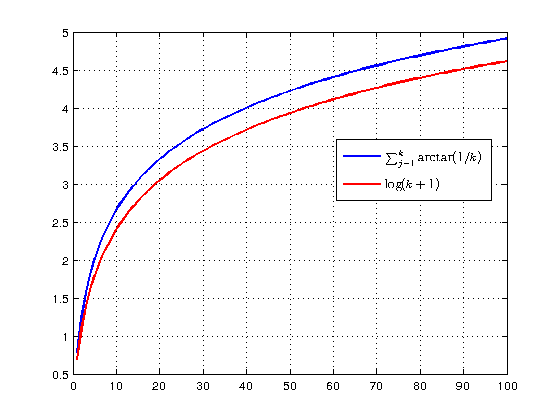
\includegraphics[width = 0.7\linewidth]{03_06_2012a.png}
\end{figure}
\fi 
The trick of proof lies with series expansion. \\

\begin{proof}
It is true for $k=1$ as $\pi/4 > \log(2)$. Now suppose the claim holds for $k-1$, i.e., $\sum_{j=1}^{k-1} \arctan\left(1/j\right) \geq \log\left(k\right)$, we need to show it holds for $k$. It suffices to show $\arctan(1/k) \geq \log\left(1+1/k\right)$. Now we consider the series expansions of $\arctan\left(x\right)$ and $\log\left(1+x\right)$: 
\begin{eqnarray*}
\arctan\left(x\right) & = x - \frac{1}{3}x^3 + \frac{1}{5}x^5 - \frac{1}{7}x^7 + \frac{1}{9}x^9 + \cdots, \forall \left|x\right|\leq 1, \\
\log\left(x+1\right) & = x - \frac{1}{2}x^2 + \frac{1}{3}x^3 - \frac{1}{4}x^4 + \frac{1}{5}x^5 + \cdots, \forall -1 < x \leq 1. 
\end{eqnarray*}
So we have
\begin{eqnarray*}
\arctan\left(x\right) - \log\left(1+x\right) & = \left(\frac{1}{2}x^2 + \frac{1}{4}x^4 + \frac{1}{6}x^6 + \cdots\right) - \left(\frac{2}{3}x^3 + \frac{2}{7}x^7 + \frac{2}{11}x^{11} + \cdots \right) \\
& = \frac{2x^2}{3}\left(\frac{3}{4}- x\right) + \frac{2x^4}{7}\left(\frac{7}{8}-x^3\right) + \frac{2x^6}{11}\left(\frac{11}{12} - x^5\right) + \cdots \geq 0
\end{eqnarray*}
if $0< x \leq \frac{3}{4}$, and $1/k, \forall k>1$ satisfies the condition.
\end{proof}

Recall that $\arctan x \leq x$. Thus we have 
\begin{equation}
\boxed{\sum_{j=1}^{k} \frac{1}{j} \geq \sum_{j=1}^{k} \arctan \frac{1}{j} \geq \log \left(k+1\right)}.
\end{equation} 
Acknowledgement: \href{http://129.81.170.14/~tamdeberhan/}{Dr. Tewodros Amdeberhan}, at Math Department of Tulane University, has kindly provided the proof and permitted me to share this on my blog. You may want to read their interesting paper on techniques of evaluating sum of arctangent: \href{http://129.81.170.14/~vhm/ac1.pdf}{Sum of Arctangents and Some Formula of Ramanujan}.  
\end{document}
